\documentclass{report}
\usepackage{amsmath}
\usepackage{amssymb}
\usepackage{amsfonts}
\usepackage{amsthm}
\usepackage[colorlinks]{hyperref}
\usepackage{listings}
\usepackage{parskip}
\usepackage{tikz}
\usepackage[margin=1.25in]{geometry}
\usetikzlibrary{positioning}
\usetikzlibrary{calc}

\newtheorem{theorem}{Theorem}

\lstdefinestyle{code}{
    language=Matlab,
    frame=L,
    basicstyle=\ttfamily,
    keywordstyle=\color{blue},
    breaklines=true
}

\renewcommand\abstractname{\textbf{Executive Summary}}

\renewcommand\appendix{\par
  \setcounter{section}{0}
  \setcounter{subsection}{0}
  \setcounter{figure}{0}
  \setcounter{table}{0}
  \renewcommand\thesection{Appendix \Alph{section}}
  \renewcommand\thefigure{\Alph{section}\arabic{figure}}
  \renewcommand\thetable{\Alph{section}\arabic{table}}
}

\title{ECE532 -- Final Project}
\author{Kyle Daruwalla \\ \href{mailto:daruwalla@wisc.edu}{daruwalla@wisc.edu}
    \and Davis Gilton \\ \href{mailto:gilton@wisc.edu}{gilton@wisc.edu}
    \and Shuoyan Qiu \\ \href{mailto:sqiu26@wisc.edu}{sqiu26@wisc.edu}
}
\date{15 Dec. 2016}

\newcommand{\set}[1]{\mathbb{#1}}
\newcommand{\rank}[1]{\mathrm{rank}\left(#1\right)}
\newcommand{\code}[1]{{\texttt{#1}}}
\renewcommand{\thesection}{\arabic{section}}

\bibliographystyle{ieeetr}

\begin{document}

\maketitle

\begin{abstract}
    This short section (about 1/2 page) should clearly explain what the project is about, which machine learning techniques are explained and utilized, and what a reader can expect to learn and accomplish if they follow along and work through the examples and problems. This is a very important part of your project, because it’s the first thing the reader sees. Be clear, be concise, and use this opportunity to convey what makes this project interesting/unique/cool.
\end{abstract}

\section{Background}
\label{sec:background}
This section should explain the context for the main idea behind the project (you may divide this section into multiple subsections if it helps with readability). Start with a description of the problem that will be solved, a brief history (with citations) of how the problem came about, why it’s important/interesting, and any other interesting facts you’d like to talk about. Feel free to use images/diagrams/etc. from research papers, the internet, or other sources to help with your explanation, so long as you cite your references. Finally, the background section should also give a mathematical description of the problem, with equations as needed.

The Singular Value Decomposition (SVD) is a popular mathematical tool, finding uses in linear algebra, signal processing, image processing, statistics, and control theory. The SVD factorizes an $m\times n$ complex matrix rank-$r$ $A$ into the form:

\[ A = U \Sigma V^\intercal \]

Where $U$ is an $m\times m$ unitary matrix and $V$ is an $n \times n$ unitary matrix. $\Sigma$ is an $m \times n$ rectangular matrix, which has only $r$ nonzero elements (called "singular values") on its diagonal, which are traditionally arranged in descending order. All other elements of $\Sigma$ are zero. So we assume $\sigma_1 \geq \sigma_2 \geq \ldots \geq \sigma_r > 0$. As usual, $r = \mathrm{rank}(A) \leq \min(m,n)$.

We call the columns of $U$, $[u_1, u_2, \ldots, u_m]$ the left singular vectors of $A$. Similarly, we refer to the columns of $V$, $[v_1, v_2, \ldots v_n]$ as the right singular vectors of $A$.

In this lab, we will also refer to the "economy" SVD. This version of the SVD factorizes $A$ as:

\[ A = U_1 \Sigma_1 V_1^\intercal \]

Where $\Sigma_1$ is an $r \times r$ diagonal matrix containing only positive singular value elements. $U_1$ is an $m \times r$ unitary matrix containing only the first $r$ left singular vectors of $A$, and $V_1$ is an $n \times r$ unitary matrix containing only the first $r$ right singular vectors of $A$. This decomposition is smaller than the full SVD, and so can be useful when dealing with extremely large matrices.

Now we can represent $A$ as a linear combination of rank-1 matrices:

\[ A = \sigma_1 u_1 v_1^\intercal + \sigma_2 u_2 v_2^\intercal + \ldots + \sigma_r u_r v_r^\intercal \]

From class, you will remember the Eckart-Young Theorem\cite{Eckart1936}:

\begin{theorem}
	Given a matrix, $A \in \set{R}^{m \times n}$ that has rank $r$, we can find a rank $k \leq r$ approximation to $A$, $X$ as
	$$\sum_{i = 1}^k \sigma_i u_i v_i^\top$$
	where $\sigma_i$ are the singular values of $A$, and $u_i$ and $v_i$ are the singular vectors of $A$. Note that $X$ is also the solution to the problem
	$$\arg \min_{\rank{B} \leq k} \|A - B\|$$
	\label{thm:eckart-young}
\end{theorem}

This tells us that the SVD can be used to find the best low-rank approximation possible. In particular, these low-rank methods can be used for image processing. 

There are many interesting applications of the SVD in image processing, including several related to Principal Component Analysis (PCA) and advanced filtering techniques.\cite{1162766}\cite{1326538}\cite{382496} The SVD can also be used on video and image data to reconstruct fragmented or damaged photos and videos.\cite{VideoRest}

In this lab, we will first explore some example image processing techniques, particularly low-rank approximations. Afterwards, we will investigate how to structure video data to be analyzable using our methods, and explore the significance of a low-rank video approximation. Finally, we will conclude with a video editing scheme based entirely around the SVD. Let's start with the warmup!

\section{Warm-Up}
\label{sec:warm-up}
The following problems are designed to familiarize you with concepts you will use throughout the lab. We will tackle four topics:
\begin{enumerate}
	\item Performing compression using the SVD on image data
	\item Working with video data in MATLAB
	\item Performing compression using the SVD on frames of video data
	\item Reshaping video data to achieve the main results of the lab
\end{enumerate}

\subsection{Compressing image data}
 Consider a grayscale image where each pixel is a value from 0 to 255. We can represent this image as a matrix of pixel values. Thm. \ref{thm:eckart-young} can be used to find a rank $r$ approximation to this matrix. Now, our image is represented by a low-rank matrix $X$, thereby compressing the image size.

\textbf{Problem:} Download the image \href{http://www.laurentlessard.com/teaching/ece532/homework/bucky.csv}{bucky.csv}. Your task is to use MATLAB and Thm. \ref{thm:eckart-young} to compress this image so it can be represented by a rank 50 matrix. Recall from a previous homework set that this will entail setting some of the singular values to 0. Solutions are included in \ref{app:warm-up-solution-1}.

\subsection{Video data in MATLAB}
So far, we've only worked with image data in MATLAB. These particular images contained only two dimensions -- width and height. Videos contain four dimensions -- width, height, channels, and time. First, a video is a series of frames in time. Each frame is still three dimensions. The third dimension, known as the channel, corresponds to the red (R), green (G), and blue (B) channels of a color image. Each channel is only two dimensions like the images we've worked so far. Previously, our image data was in grayscale, which is only one channel instead of three. In order to perform the problems in this lab, we will need to convert the video data from color to grayscale.

\textbf{Problem:} Use the code snippet below to read in a video built in to MATLAB. Then go through the video frame-by-frame and convert it from RGB to grayscale. (\textit{Hint:} you might find the MATLAB documentation on \code{VideoReader}, \code{rgb2gray}, and \code{implay} helpful). Solutions are included in \ref{app:warm-up-solution-2}.
\begin{lstlisting}[style=code]
v = VideoReader('xylophone.mp4');
videoMatrix = v.read;
\end{lstlisting}

\subsection{Compressing frame by frame}
Based on the previous two problems, the obvious next step to applying SVD compression to video data might be to apply it frame by frame.

\textbf{Problem:} Use your result from the previous warm-up problem to compress the grayscale video frame by frame. Use the same compression value ($k = 50$). What do you notice about the output? Is it as you expected? Try it with a lower compression value ($k = 20$) to see more drastic results. Solutions are included in \ref{app:warm-up-solution-3}.

\subsection{Reshaping video data}
This problem is a simple thought experiment. As shown in Fig. \ref{fig:warm-up-4-experiment}, we have a viewing window frame (represented by the red box), and we are sliding a $1\text{px} \times 1\text{px}$ black square across the screen. Ignore the numbers in Fig. \ref{fig:warm-up-4-experiment} for now.
\begin{figure}[ht]
	\centering
	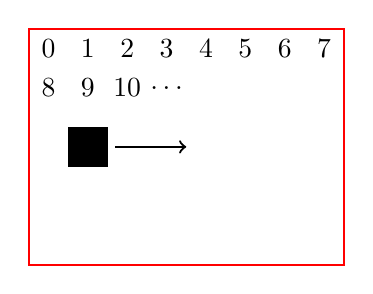
\begin{tikzpicture}
		\draw [red, thick] (0, 0) rectangle (4, -3);
		\draw [fill] (0.5, -1.25) rectangle (1, -1.75);
		\draw [->, thick] (1.1, -1.5) -- (2, -1.5);

		\foreach \i in {0, ..., 7} {
			\node at (0.5*\i + 0.25, -0.25) {\i};
		}

		\foreach \i in {0, ..., 2} {
			\pgfmathtruncatemacro{\j}{\i + 8};
			\node at (0.5*\i + 0.25, -0.75) {\j};
		}

		\node at (1.75, -0.75) {$\ldots$};
	\end{tikzpicture}
	\caption{The red box is the viewing frame of the video capture device. The black square moves under the viewing frame from left to right.}
	\label{fig:warm-up-4-experiment}
\end{figure}

\textbf{Problem:} Focus on the pixel at (0, 0). What single value represents its value over all of time? Now focus on a pixel in the same row as the black box. If you had to guess at a random time what its value was, what would be the best value to guess? (\textit{Hint:} don't over think it or actually calculate the average).

Now suppose you vectorize the 2D viewing window -- count across the pixels in the frame as shown in Fig. \ref{fig:warm-up-4-experiment} and place them in a row vector in that order. Suppose there are $N$ total pixels in the frame, then the row vector should be $1 \times N$. This vector represents the values of all the pixels at one moment in time. Now create another such row vector for the next moment in time, and so on, until you have $T$ $1 \times N$ vectors. Arrange these vectors in a matrix so that each row of the matrix is one of the row vectors, and as you go down the rows of the matrix, you are advancing in time. Note that each \textit{column} of this matrix is the values of a single pixel across all values of time. What would this matrix look like for the experiment in Fig. \ref{fig:warm-up-4-experiment}? You can now choose a \textit{column} vector to represent all the columns of this matrix. What vector do you choose?

The standard way to reshape a matrix into a vector is to ``stack'' the columns so that the matrix ($M \times N$) becomes an $MN \times 1$ column, with the first column of our matrix on top, the second immediately below it, and so on. We will use this method for reshaping videos in this lab.

\section{Lab}
\label{sec:lab}
\subsection{Setup}

During the course of this lab we will operate on the ``xylophone.mp4'' video that you used in the warm-up section.

If you have not already done so, use the code developed in Warm-Up Problem 2 to read in the ``xylophone.mp4'' video and convert it to grayscale. After Warm-Up Problem 4, you should have a good idea of how to reshape the data to make the three-dimensional video data into two dimensions. Convert the 3-D grayscale video matrix into a 2-D matrix.

(\textit{Hint:} Ensure that the resulting 2-D matrix has the same number of columns as there are frames in the video, and $320 \times 240$ rows)

Test that you can recreate the original grayscale video using only the results of the SVD.

\subsection{SVD and Eckart-Young With Video Data}

We will now take the SVD of the video data, to try to see what a low-rank approximation of a video might look like. As we saw in Warm Up Problem 3, computing the SVD for every frame is a valid approach, but doesn't produce any effects unique to videos. So we want to find a way to compute the SVD across an entire video.

The SVD is only defined for 2-D matrices, so we have to use the flattened matrix we created in Lab Problem 1.

Should you take the economy SVD, or the full SVD? What will be the dimensions of the resulting U, S, and V matrices in both cases? How much storage space would these matrices require?

In the Warm-Up Problem 1, you reviewed how to do a low-rank approximation of image data. There, you let $k = 20$. Here, let $k = 6$, and reconstruct an approximation to ``xylophone.mp4'' letting only the first 6 singular values be nonzero.

Convert this into a video, and watch the video using MATLAB's \code{implay()} function (remember that you need to convert the data to \code{uint8} before watching the video!). What do you observe? Why might this be?

Given another video, what would you expect a very low-rank approximation of that video to look like?

\subsection{Inverse Eckart-Young?}

In the previous problem, we were able to extract the low-rank approximation to our video data. In practice what this ended up meaning is that we removed those objects in the video that weren't constant over the time dimension -- they were moving.

The result was extracting only the background. But what happens to the moving objects (and the lighting changes)? Which singular values would you set to zero to extract only the objects in the video that are moving?

Using the results of the SVD that you took in Lab Problem 2, extract the moving parts of ``xylophone.mp4'' and convert them back into a video. Play back the video to ensure that your method worked.

\subsection{Video Editing with the SVD}

We now have all the tools we need to do some simple video editing. The conclusion of our lab will be using the ideas we have developed so far to replace the background of our ``xylophone.mp4'' video.

This can be done with any image of appropriate size, as long as that image is grayscale and $240 \times 320$ pixels. MATLAB has a built-in image that can be used for this purpose when downsampled using the following code snippet:

\begin{lstlisting}[style=code]
backgroundImage = imread('AT3_1m4_03.tif');
backgroundImage = downsample(downsample(backgroundImage,2)',2)';
\end{lstlisting}

Reshape this image, and then take the SVD as if it were a single-frame video. The reshaped image should be a single column vector. What size do you expect your U, S, and V matrices to be? After taking the SVD, did the result make sense?

Because this is a single-frame video, the $V$ vector is $1\times 1$. Is there a way to make this $V$ vector more closely resemble the $V$ vector produced when taking the SVD of the ``xylophone.mp4'' data?
(\textit{Hint:}  You could create a video where every frame was this image; what would your $V$ vector look like in that case?)

Replace the first left singular vector of the ``xylophone.mp4'' 2D matrix with the $U$ from our image. Similarly, replace the right singular vector with the $V$ vector you just created. You should also replace the top singular value with the singular value you obtained in this problem.

Recreate and play the new video. What do you observe?

Experiment. Can you remove the xylophone keys, but leave the arm and stick? How about the other way around?





\nocite{*}
\bibliography{references}

\newpage
\appendix
\section{Solutions}
\label{app:solutions}
This appendix contains solutions to the warm-up problems and lab.

\subsection{Warm-Up Solution \#1}
\label{app:warm-up-solution-1}
The code below will produce a rank 50 approximation to the original image. Notice how the image is blurred from compression. Play with the value of $k$ and see what the results look like.
\lstinputlisting[style=code,title=WarmUp1.m]{../Code/WarmUp1.m}

The image that should be produced is:

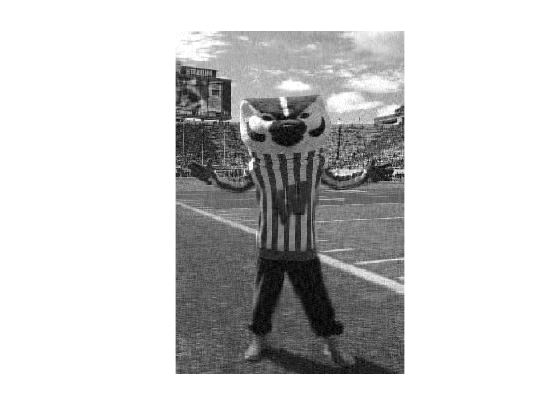
\includegraphics[scale=0.75]{../Report/bucky50.png}

\subsection{Warm-Up Solution \#2}
\label{app:warm-up-solution-2}
The code below reads in a video file and converts each frame from RGB to grayscale.
\lstinputlisting[style=code,title=WarmUp2.m]{../Code/WarmUp2.m}

\subsection{Warm-Up Solution \#3}
\label{app:warm-up-solution-3}
The code below will compute video compression by doing standard SVD image compression on each frame individually. It uses a compression value of $k = 20$, but the value of $k$ can be changed in the code easily to compute the output for different compression values.
\lstinputlisting[style=code,title=WarmUp3.m]{../Code/WarmUp3.m}

When we performed compression on images, the results just looked like lower resolution images. The video compression results appear to have a similar characteristic. So far, this makes sense, but it doesn't appear to target low frequency or high frequency portions of the video like we wanted. However, if you bump up the compression to $k = 20$, then the video doesn't just look like it is lower resolution, but it is also blurry (almost as if someone used the smudge tool in Photoshop on it). This is because we are compressing frames individually and not relating them to each other. The next warm-up exercise will help you explore how we can apply the same SVD techniques across the time dimension.

Videos can be found at:

\text{https://github.com/NiceanLoH/videoData/blob/master/compressed\_video\_20.zip}

\text{https://github.com/NiceanLoH/videoData/blob/master/compressed\_video\_50.zip}

\subsection{Warm-Up Solution \#4}
\label{app:warm-up-solution-4}
For the thought experiment, the pixel at (0, 0) is white for all time, so we can use the value 0 to represent it. Similarly, a pixel in the same row as the black box is white almost all of the time, except it is black for one time instance. Therefore, we can just use a pixel value of 0 to represent it, and we would be write most of the time.

The matrix we are trying to form looks like this:
$$\left[\begin{matrix}
	0 & 0 & \ldots & 0 & 0 \\
	0 & 1 & \ldots & 0 & 0 \\
	\vdots & \vdots & \vdots & \vdots & \vdots \\
	0 & 0 & \ddots & 0 & 0 \\
	0 & 0 & \ldots & 1 & 0 \\
	0 & 0 & \ldots & 0 & 0
\end{matrix}\right]$$
It is a matrix with a small identity matrix in the center that is surrounded by zeros all around. If we look at each column of this matrix, it is either all zeros, or it is zeros everywhere except one element is one. If we can only use one vector to represent these vectors, we would choose a vector of all zeros, because placing a single 1 in any position would only be correct for one column and wrong for all others.

Notice that this matrix has reduced an entire video to just two dimensions -- position along the columns and time along the rows. Applying the SVD techniques to this matrix will do what we have been doing in this warm-up exercise -- it tries to use a single vector to represent several positions in the image across time. These vectors may not be all ones or zeros like we have been constructing. Think about positions in the image whose \textit{change} over time is similar. The background pixel positions are all subject to the same change over time (lighting, etc). So, a single unit vector can represent that normalized change. Then each pixel is just a scalar multiple of that vector. So what does using the SVD to find a low-rank approximation to this matrix do? Simply, it tries to represent the matrix using only a few basis vectors. The number of basis vectors is the determined by the rank chosen for the low-rank approximation.

\end{document}